
\documentclass{beamer}


\mode<presentation> 
	{
	%\usetheme{Berlin}
	%\usetheme{Copenhagen}
	%\usetheme{Luebeck}
	\usetheme{Madrid}
	\setbeamertemplate{navigation symbols}{} 
	\setbeamertemplate{itemize item}[square]
	\setbeamertemplate{itemize subitem}[square]
	\setbeamertemplate{caption}{\raggedright\insertcaption\par}
	\setbeamerfont{footnote}{size=\tiny}

	%\makeatletter
	\setbeamercolor{footline}{fg=white, bg=darkblue}
	\setbeamertemplate{footline}
	{
	  \leavevmode%
	  \hbox{%
	  \begin{beamercolorbox}[wd=.25\paperwidth,ht=2.25ex,dp=1ex,center]{footline}%
	    \usebeamerfont{author in head/foot}\insertauthor\hspace*{1em}
	  \end{beamercolorbox}%
	  \begin{beamercolorbox}[wd=.50\paperwidth,ht=2.25ex,dp=1ex,center]{footline}%
	    \usebeamerfont{title in head/foot}\insertshorttitle
	  \end{beamercolorbox}%
	  \begin{beamercolorbox}[wd=.25\paperwidth,ht=2.25ex,dp=1ex,right]{footline}%
	    \usebeamerfont{date in head/foot}\insertshortdate{}\hspace*{2em}
	  \end{beamercolorbox}}%
	  \vskip0pt%
	}
	%\makeatother

	}

\usepackage{graphicx} 
\usepackage{booktabs}
\usepackage{textcomp} 
\usepackage{braket}
\usepackage{comment}

\usepackage{tcolorbox}
\usepackage{amsmath,amssymb}

\newcommand\blfootnote[1]{%
  \begingroup
  \renewcommand\thefootnote{}\footnote{#1}%
  \addtocounter{footnote}{-1}%
  \endgroup
}

\definecolor{darkblue}{RGB}{32, 76, 129}
\definecolor{darkish_blue}{RGB}{32, 76, 157}

\setbeamercolor{frametitle}{bg=darkblue, fg=white}

\newcommand{\bb}[1]{\textbf{\textcolor{darkish_blue}{#1}}}




%----------------------------------------------------------------------------------------
%	TITLE PAGE
%----------------------------------------------------------------------------------------

\title[Quantum walks with time-dependent Hamiltonians]{Quantum walks with time-dependent Hamiltonians  \\ and their application to the search problem on graphs} 

\author{Matteo Garbellini} 
\institute[(UniMi)] 
{
Universit\`a degli Studi di Milano \\ 
\medskip
}
\date{12 Ottobre 2020} 

\begin{document}

%----------------------------------------------------------------------------------------
%	PRESENTATION SLIDES
%----------------------------------------------------------------------------------------

%\begin{frame}
%\frametitle{Overview}
%\tableofcontents
%\end{frame}

%------------------------------------------------

\begin{frame}
\frametitle{Unstructured search problem}
\begin{itemize}
	\item $N$ items $\{1, 2,..., N\}$
	\item One "marked item" $w$ represents the solution
	\item Query: "is $w=x$?" is a black box function
\end{itemize}
\begin{figure}
	\centering
	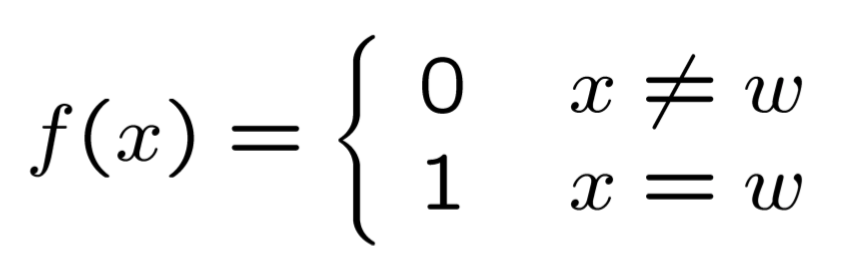
\includegraphics[width=4cm]{black_box.png}
\end{figure}
\begin{itemize}
	\item \bb{Classical}: $O(N)$
\end{itemize}

\end{frame}

%------------------------------------------------

\begin{frame}
\frametitle{Grover's quantum search}

\begin{columns}
	\begin{column}[T]{0.5\textwidth}
		\begin{itemize}
			\item Takes advantage of the \bb{superposition} of states
			\item Algorithm consists in repeated application of the \bb{Grover's operator} $U_G = U_\psi U_w$
			\item \bb{Oracle $U_w$}: a black box that \bb{marks} the solution with a phase
			
		\end{itemize}

		\vspace{1.5cm}
		\begin{itemize}
			\item \bb{Quantum Grover}: $O(\sqrt{N})$
		\end{itemize}
	\end{column}

	\begin{column}[T]{0.4\textwidth}
	\vspace{-0.2cm}
	\begin{tcolorbox}[width=5.2cm, colframe=darkblue, colback=white, halign=center, left=1pt, right=1pt]
	\centering
	\bb{Search procedure}
		\begin{itemize}
			\item Preparation of the superposition state $$\ket{\psi}=\frac{1}{\sqrt{N}}\sum_{x}\ket{x}$$ 
			\item Oracle application $$\ket{x}\xrightarrow{U_w}(-1)^{f(x)}\ket{x}$$
			\item Application of $U_\psi$ $$2\ket{\psi}\bra{\psi}-I$$
			\item Readout
		\end{itemize}
	\end{tcolorbox}
	\end{column}

\end{columns}
\end{frame}

%------------------------------------------------

\begin{frame}
\frametitle{Spatial search by quantum walks}

\begin{columns}
	\begin{column}[T]{0.50\textwidth}
		\begin{itemize}
			\item $N$ elements distributed in space, described by \bb{$N$-vertex graph} 
			\item Quantum walk dynamics determined by the \bb{Laplacian} $L$ of the graph 
			\item Marked state is \bb{identified} by an \bb{oracle} $ H_w = -\ket{w}\bra{w}$ 
		\end{itemize}

		\vspace{0.3cm}
		\centering
		\begin{tcolorbox}[width=4.0cm, colframe=darkblue, colback=white, halign=center, left=1pt, right=1pt, top=-11pt, bottom=1pt]
			\begin{equation*}
				H=-\gamma L -\ket{w}\bra{w}
			\end{equation*}
		\end{tcolorbox}



		\vspace{0.5cm}
		\begin{itemize}
			\item \bb{Complete graph}: $O(\sqrt{N})$
		\end{itemize}
	\end{column}

	\begin{column}[T]{0.4\textwidth}
	\vspace{-0.2cm}
	\begin{tcolorbox}[width=5.0cm, colframe=darkblue, colback=white, halign=center, left=1pt, right=1pt]
	\centering
	\bb{Search procedure}
		\begin{itemize}
			\item Start in state $\ket{s} = \frac{1}{\sqrt{N}}\sum_{j}\ket{j}$
			\item Schroedinger evolve for time $T$ using the Hamiltonian $H$
			\item Measure the state
			\item Goal: choose $\gamma$, $T$ so that the probability $|\braket{w|e^{-iHT}|s}|^2$ is as close to $1$ for the smallest $T$.
		\end{itemize}
	\end{tcolorbox}
	\end{column}

\end{columns}

\vspace{0.5cm}
\footnotesize A. Child and J. Goldstone, Spatial search by quantum walk. \textit{Physical Review A} (2004)
\end{frame}

%------------------------------------------------


\begin{frame}
\frametitle{Search by quantum walks}

\begin{columns}

	\begin{column}[T]{0.5\textwidth}
		\begin{itemize}
			\item $N$ elements distributed in space (e.g., a physical database)
			\item Model: $N$-vertex graph $G$
			\item Dynamics of the quantum walk on the graph is determined by the Laplacian $L$ of the graph $$H=-\gamma L$$
		\end{itemize}
	\end{column}

	\begin{column}[T]{0.4\textwidth}
	\vspace{-0.2cm}
	\begin{tcolorbox}[width=5.2cm, colframe=darkblue, colback=white, halign=center, left=1pt, right=1pt, top=1pt, bottom=3pt]
		\footnotesize
		\begin{figure}
			
			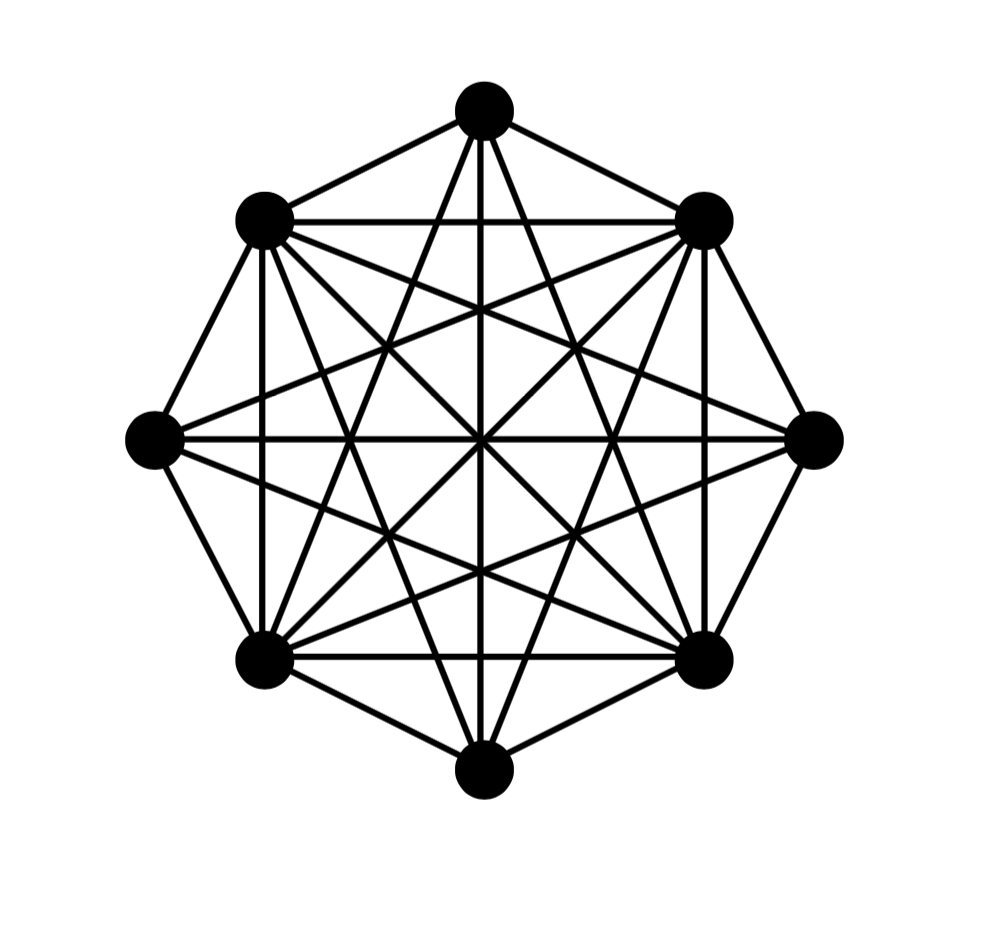
\includegraphics[width=0.6\textwidth]{complete_graph.png}
		\end{figure}
		\vspace{-0.7cm}
		\bb{Adjacency matrix}:
		\begin{equation*}
			A_{ij} = \begin{cases} 1 & \mbox{if }(i,j)\in G \\ 0 & \mbox{otherwise} \end{cases}
		\end{equation*}
		\bb{Diagonal degree matrix}:
		\begin{equation*}
			D_{jj}= deg(j)
		\end{equation*}
		\bb{Laplacian matrix}:
		\begin{equation*}
			L = A-D
		\end{equation*}
	\end{tcolorbox}
	\end{column}

\end{columns}
\end{frame}

%------------------------------------------------
\begin{comment}
\begin{frame}
\frametitle{Search by quantum walks (2)}

\begin{itemize}
	\item Marked state is identified by an "oracle Hamiltonian" $ H_w = -\ket{w}\bra{w}$ 
\end{itemize}

\begin{equation*}
	H = \gamma L - \ket{w}\bra{w}
\end{equation*}

\hspace{0.5cm}\bb{Search procedure}
\begin{itemize}
	\item Start in state $\ket{s} = \frac{1}{\sqrt{N}}\sum_{j}\ket{j}$
	\item Schroedinger evolve for time $T$ using the Hamiltonian $H$
	\item Measure the state
	\item Goal: choose $\gamma$, $T$ so that the probability $|\braket{w|e^{-iHT}|s}|^2$ is as close to $1$ for the smallest $T$.
\end{itemize}

\vspace{0.3cm}
\centering
\begin{tcolorbox}[width=6.5cm, colframe=darkblue, colback=white, halign=center, left=1pt, right=1pt]
\large For the \bb{complete graph} a time scaling of $O(\sqrt{N})$ can be achieved
\end{tcolorbox}

\vspace{0.5cm}
\footnotesize A. Child and J. Goldstone, Spatial search by quantum walk. \textit{Physical Review A} (2004)
\end{frame}
\end{comment}
%------------------------------------------------

\begin{frame}
\frametitle{Search by adiabatic evolution}

\vspace{-0.3cm}
\begin{itemize}
	\item The \bb{adiabatic theorem} ensures that under certain conditions if a system evolves slow enough, it remains in its ground state
	\item It is used to solve computational problem via a \bb{time-dependent evolution}: 
\end{itemize}
\centering
\begin{tcolorbox}[width=4.0cm, colframe=darkblue, colback=white, halign=center, left=1pt, right=1pt, top=-11pt, bottom=1pt]
	\begin{equation*}
		H(s) = (1-s)H_i + sH_f
	\end{equation*}
\end{tcolorbox}

\vspace{0.5cm}
\begin{columns}

	\begin{column}[T]{0.4\textwidth}
	\bb{Global adiabatic search}
	\begin{itemize}
		\item Adiabatic theorem is applied globally
		\item Linear $s(t)$
		\item Time scaling: $O(N)$
	\end{itemize}
	\end{column}

	\begin{column}[T]{0.4\textwidth}
	\bb{Local adiabatic search}
	\begin{itemize}
		\item Adiabatic theorem is applied locally
		\item Non-linear $s(t)$
		\item Time scaling: $O(\sqrt{N})$
	\end{itemize}
	\end{column}

\end{columns}

\vspace{0.8cm}
\footnotesize J. Roland and N. Cerf, Quantum search by local adiabatic evolution. \textit{Physical Review A}
\end{frame}

%------------------------------------------------

\begin{frame}
\frametitle{Impossibility of adiabatic quantum walk search}

\begin{itemize}
	\item Both approches individually perform well, what happens if we combine them? \vspace{0.6cm}
	\item Wong \textit{et. al} (2016) showed that is is \bb{impossible} to construct an \bb{adiabatic-quantum walk} search algorithm (for the complete graph)
	\item It would need a stronger structure than the Grover's oracle
\end{itemize}

\vspace{0.5cm}
{
\centering
\begin{tcolorbox}[width=9cm, colframe=darkblue, colback=white, halign=center, left=1.5pt, right =1.5pt]
\large It leaves space for a time-dependent approach \bb{inspired} by the adiabatic evolution, but \bb{free} from the \bb{constraints} of the adiabatic theorem
\end{tcolorbox}
}

\vspace{0.5cm}
\footnotesize T. Wong and D. Meyer, Irreconcilable difference between quantum walks and adiabatic quantum computing. \textit{Physical Review A} (2016)
\end{frame}

%------------------------------------------------

\begin{frame}
\frametitle{Time-dependent Hamiltonian}
\vspace{-0.5cm}
\begin{itemize}
	\item We consider a time-dependent Hamiltonian \bb{inspired} by the adiabatic evolution
\end{itemize}
\begin{equation*}
	H(s) = (1-s)L - s\gamma\ket{w}\bra{w} 
\end{equation*}
\hspace{0.8cm}where $L$ is the \bb{Laplacian} of the graph, $s$ is the \bb{interpolating\\\hspace{0.8cm}schedule} and $\ket{w}\bra{w}$ is the \bb{oracle} Hamiltonian

\vspace{0.5cm}
\begin{itemize}
	\item The evolution of the state is determined by solving the schroedinger equation
\end{itemize}
\begin{equation*}
	i\frac{d}{dt}\ket{\psi(t)} = H\ket{\psi(t)}
\end{equation*}
\hspace{0.8cm}with the necessary boundary conditions.

\end{frame}

%------------------------------------------------

\begin{comment}
\begin{frame}
\frametitle{Interpolating schedule s(t)}

\begin{itemize}
	\item Plays a crucial role in the evolution of the system
	\item For the local adiabatic evolution a \bb{non-linear} interpolating schedule is used
	\item We take the key aspects and consider a similar non-linear s(t)
\end{itemize}

\begin{columns}
	\begin{column}[T]{0.35\textwidth}
	\centering
	\vspace{1.1cm}
		\begin{equation*}
			s_{NL}(t) = \frac{1}{2}\Big[\Big(2\frac{t}{T}\Big)^3 +1\Big]
		\end{equation*}
	\end{column}
	\begin{column}[T]{0.5\textwidth}
	\centering
		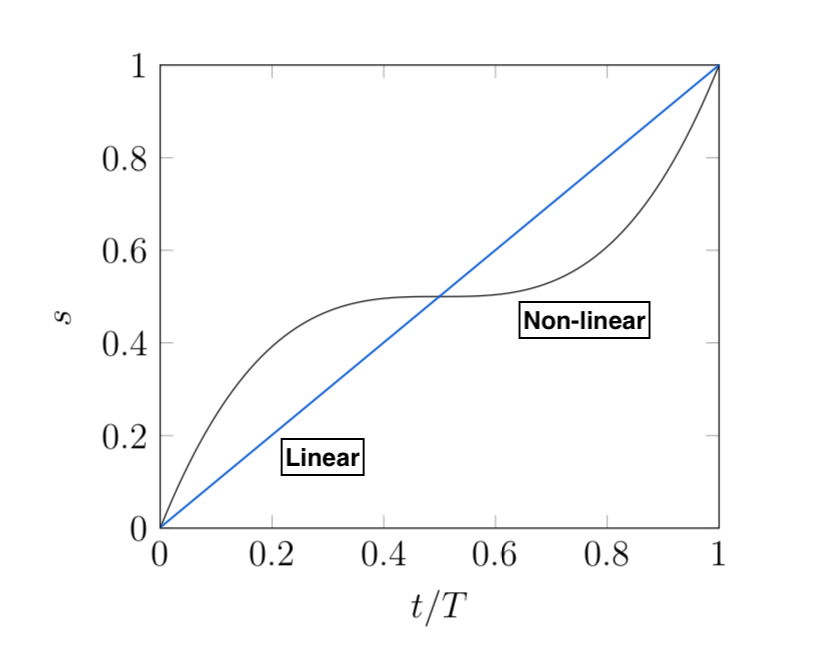
\includegraphics[width=\textwidth]{interpolating_schedule.png}

	\end{column}
\end{columns}
\end{frame}
\end{comment}
%------------------------------------------------

\begin{frame}
\frametitle{Interpolating schedule and multiple runs for one search}
\begin{columns}
	\begin{column}[T]{0.45\textwidth}
		\vspace{0.75cm}
		\begin{itemize}
			\item We considered  \bb{linear} $s_L(t)$ and \bb{non-linear} $s_{NL}(t)$ interpolating schedules
		\end{itemize}
	\end{column}
	\begin{column}[T]{0.45\textwidth}
		\vspace{-0.75cm}
		\begin{figure}
			\centering
			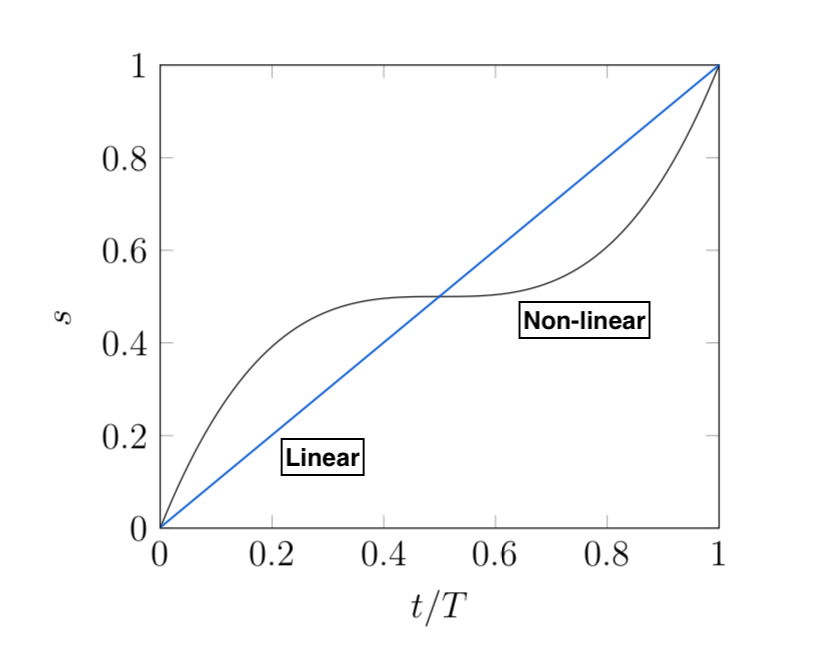
\includegraphics[width=\textwidth]{interpolating_schedule.png}
		\end{figure}
	\end{column}

\end{columns}


\begin{itemize}
	\item If the search is \bb{imperfect} (solution found with $p<1$) we consider the possibility of repeating the search \bb{multiple times}
\end{itemize}
\end{frame}

%------------------------------------------------

\begin{frame}
\frametitle{Selected graphs: cycle and complete}



\begin{columns}
	\begin{column}[T]{0.4\textwidth}
	\vspace{-0.7cm}
		\begin{figure}
			\centering
			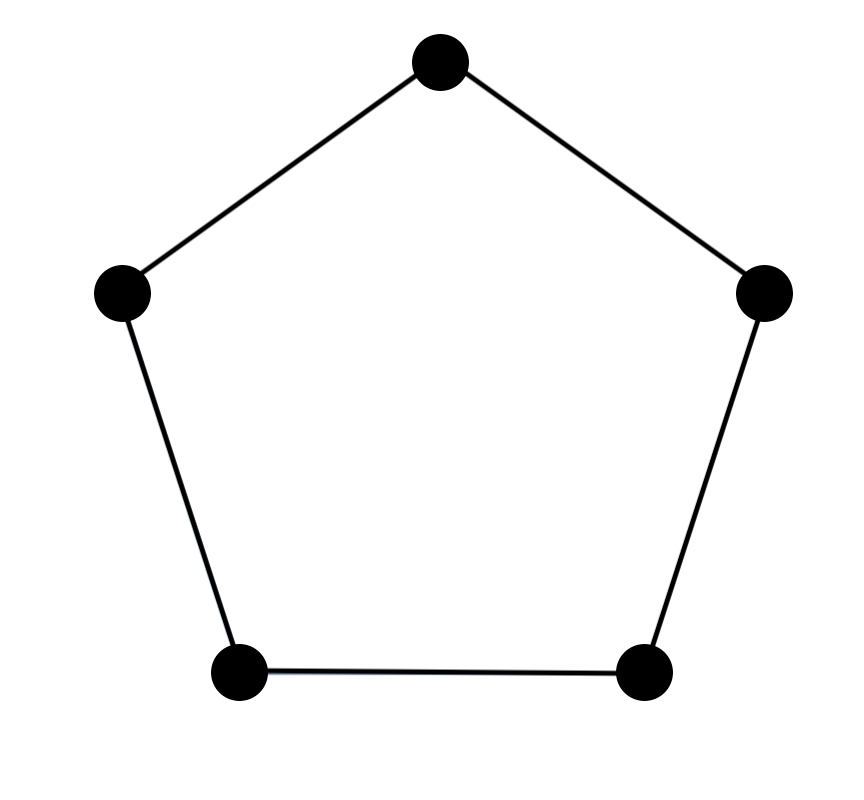
\includegraphics[width=0.5\textwidth]{cycle.png}
		\end{figure}
	\vspace{-0.5cm}
	\bb{Cycle graph $Cy(N)$}\\
	Worst case scenario
	\begin{itemize}
		\item Search problem is \bb{not solved} with the standard quantum walks approach
	\end{itemize}
	\end{column}

	\begin{column}[T]{0.4\textwidth}
	\vspace{-0.7cm}
		\begin{figure}
			\centering
			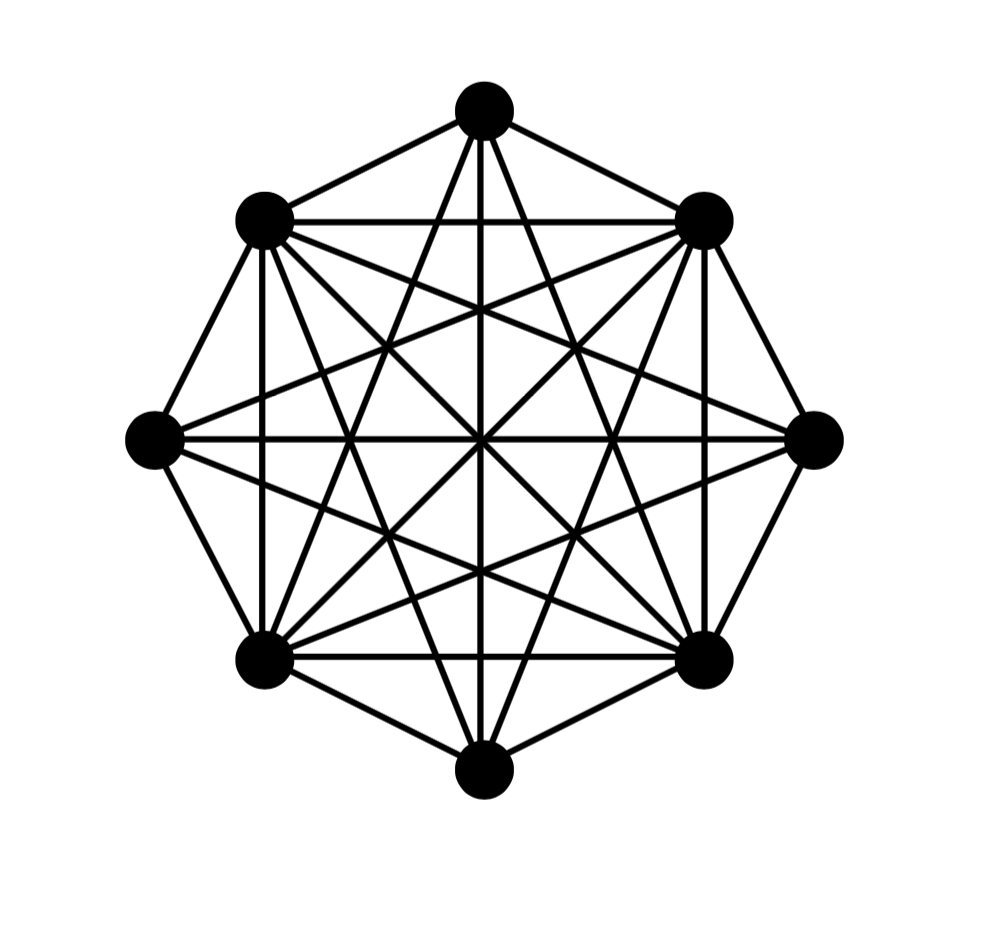
\includegraphics[width=0.5\textwidth]{complete_graph.png}
		\end{figure}
	\vspace{-0.5cm}
	\bb{Complete graph $C(N)$}\\
	Best case scenario
	\vspace{0.3cm}
	\begin{itemize}
		\item Search problem \bb{solved} with standard quantum walks approach
		\item The equivalent \textit{unstructured search} is \bb{solved} with the local adiabatic evolution
	\end{itemize}
	\end{column}
\end{columns}

\end{frame}

%------------------------------------------------

\begin{frame}
\frametitle{Results characterization: search, localization and robustness}
\vspace{-0.25cm}
\begin{columns}
	\begin{column}[T]{0.4\textwidth}
	\bb{Search}\\Finding of the solution with high probability for the \bb{smallest} $T$ possible

	\end{column}

	\begin{column}[T]{0.4\textwidth}
	\bb{Localization}\\Finding of the solution with high probability \bb{without} the need to \bb{minimize} the time
	
	\end{column}
\end{columns}

\vspace{0.5cm}
\centering
\begin{tcolorbox}[width=9cm, colframe=darkblue, colback=white, halign=center, left=0pt, right =0pt, top=1pt, bottom=1pt]
A description of the \bb{localization} is necessary given\\ the \bb{adiabatic nature} of the algorithm
\end{tcolorbox}
\vspace{0.5cm}

\begin{columns}
	\begin{column}[T]{0.4\textwidth}
		\bb{Robustness $R_\gamma$ and $R_T$} \\Quantifies the variation of the probability due to variation of $\gamma$ and $T$

	\end{column}

	\begin{column}[T]{0.4\textwidth}
		\begin{equation*}
			R^\pm = p(T,\gamma)-p(T, \gamma \pm \delta)
		\end{equation*}
		\begin{equation*}
			R_\gamma = \Big[\frac{R^++R^-}{2}\Big]
		\end{equation*}
	
	\end{column}
\end{columns}

\end{frame}

%------------------------------------------------

\begin{comment}
\begin{frame}
\frametitle{Results characterization: robustness}

\vspace{-0.5cm}
\begin{itemize}
	\item The maximum probability is produced by the optimal $\gamma$, $T$ combination
	\item If $T$ and $\gamma$ are affected by noise they might lead to variation of the probability
	\item The \bb{robustness} quantifies the variation of $p$ due to noise on $\gamma$ and $T$
\end{itemize}

\vspace{0.5cm}
\begin{columns}

	\begin{column}[T]{0.4\textwidth}
		\centering
		\bb{$\gamma$-Robustness}
		\begin{equation*}
			R^\pm = p(T,\gamma)-p(T, \gamma \pm \delta)
		\end{equation*}
		\begin{equation*}
			R_\gamma = \Big[\frac{R^++R^-}{2}\Big]
		\end{equation*}
	\end{column}

	\begin{column}[T]{0.4\textwidth}
		\centering
		\bb{$T$-Robustness}
		\begin{equation*}
			R^\pm = p(T,\gamma)-p(T\pm\tilde{\delta}, \gamma)
		\end{equation*}
		\begin{equation*}
			R_T = \Big[\frac{R^++R^-}{2}\Big]
		\end{equation*}
	\end{column}

\end{columns}

\end{frame}
\end{comment}

%------------------------------------------------

\begin{frame}
\frametitle{Cycle graph: probability grid evaluation}

\centering
\begin{tcolorbox}[width=10cm, colframe=darkblue, colback=white, halign=center, left=0pt, right =0pt]
\large We compared the \bb{time-independent} approach and the\\ \bb{time-dependent} one with \bb{linear} and \bb{non-linear} $s(t)$
\end{tcolorbox}

\begin{itemize}
	\item Computed the probability over a \bb{grid} for the different combination of $T$ and $\gamma$, with graphs up to $N=71$
\end{itemize}
\begin{itemize}
	\item Intuitive way to visualize the results: \bb{probability heatmaps}\\ \footnotesize(in figure  $N=51$)
\end{itemize}
\begin{figure}
	\centering
	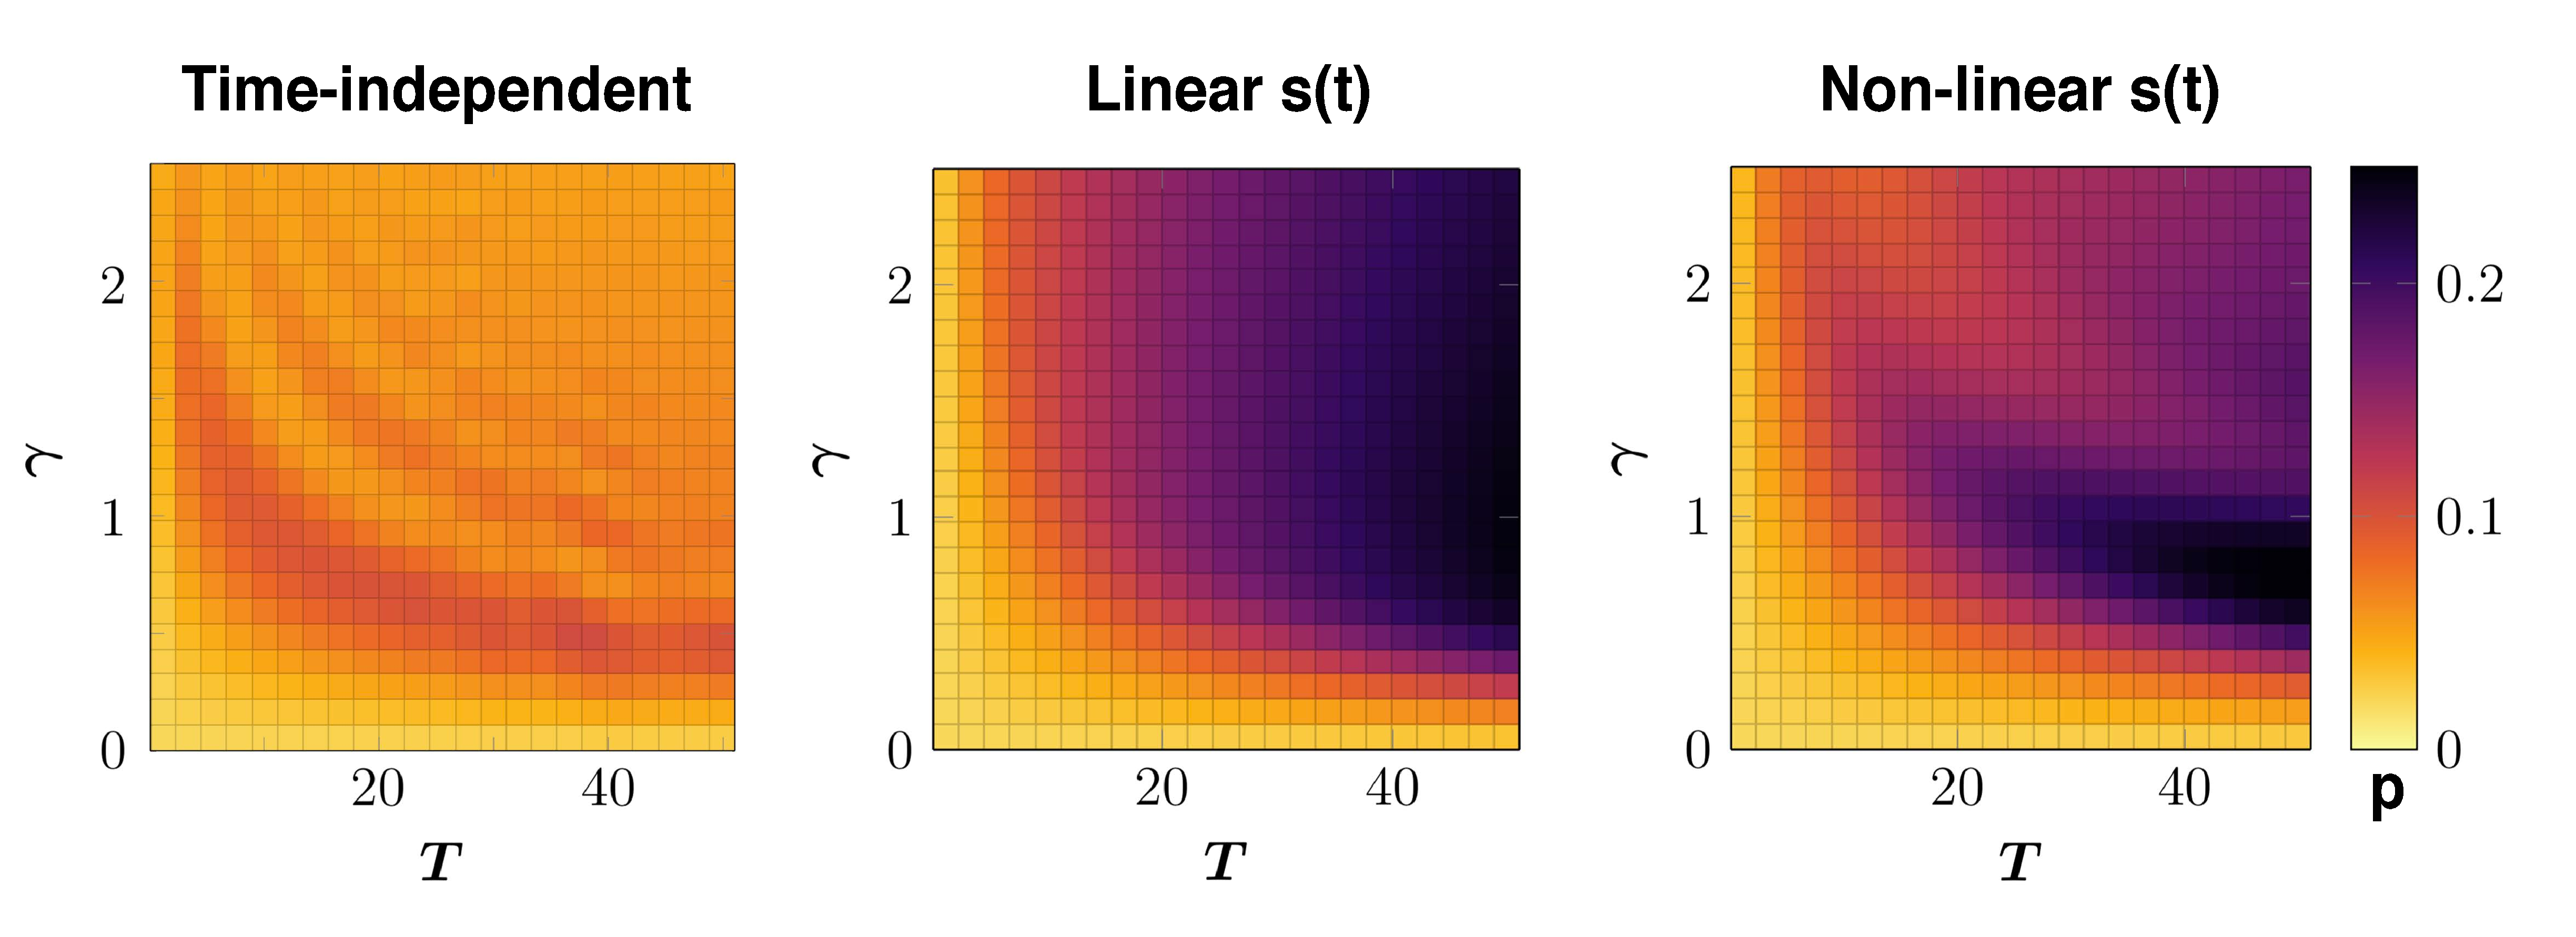
\includegraphics[width=0.8\textwidth]{heatmap_plots.pdf}
\end{figure}

\end{frame}

%------------------------------------------------

\begin{frame}
\frametitle{Cycle graph: localization \\ \normalsize $\blacksquare$ Time-dependent approach shows localization properties}

\begin{columns}
	\begin{column}[T]{0.5\textwidth}
		\vspace{0.5cm}
		\begin{itemize}
			\item The time-independent approach (red) does \bb{not} have \bb{localization} properties		
		\end{itemize}
		\vspace{0.3cm}
		\begin{itemize}
			\item The time-dependent approach (green) is able to achieve $p=1$, although for \bb{large} $T$ ($\approx N^2$)
		\end{itemize}
		
	\end{column}

	\begin{column}[T]{0.5\textwidth}
		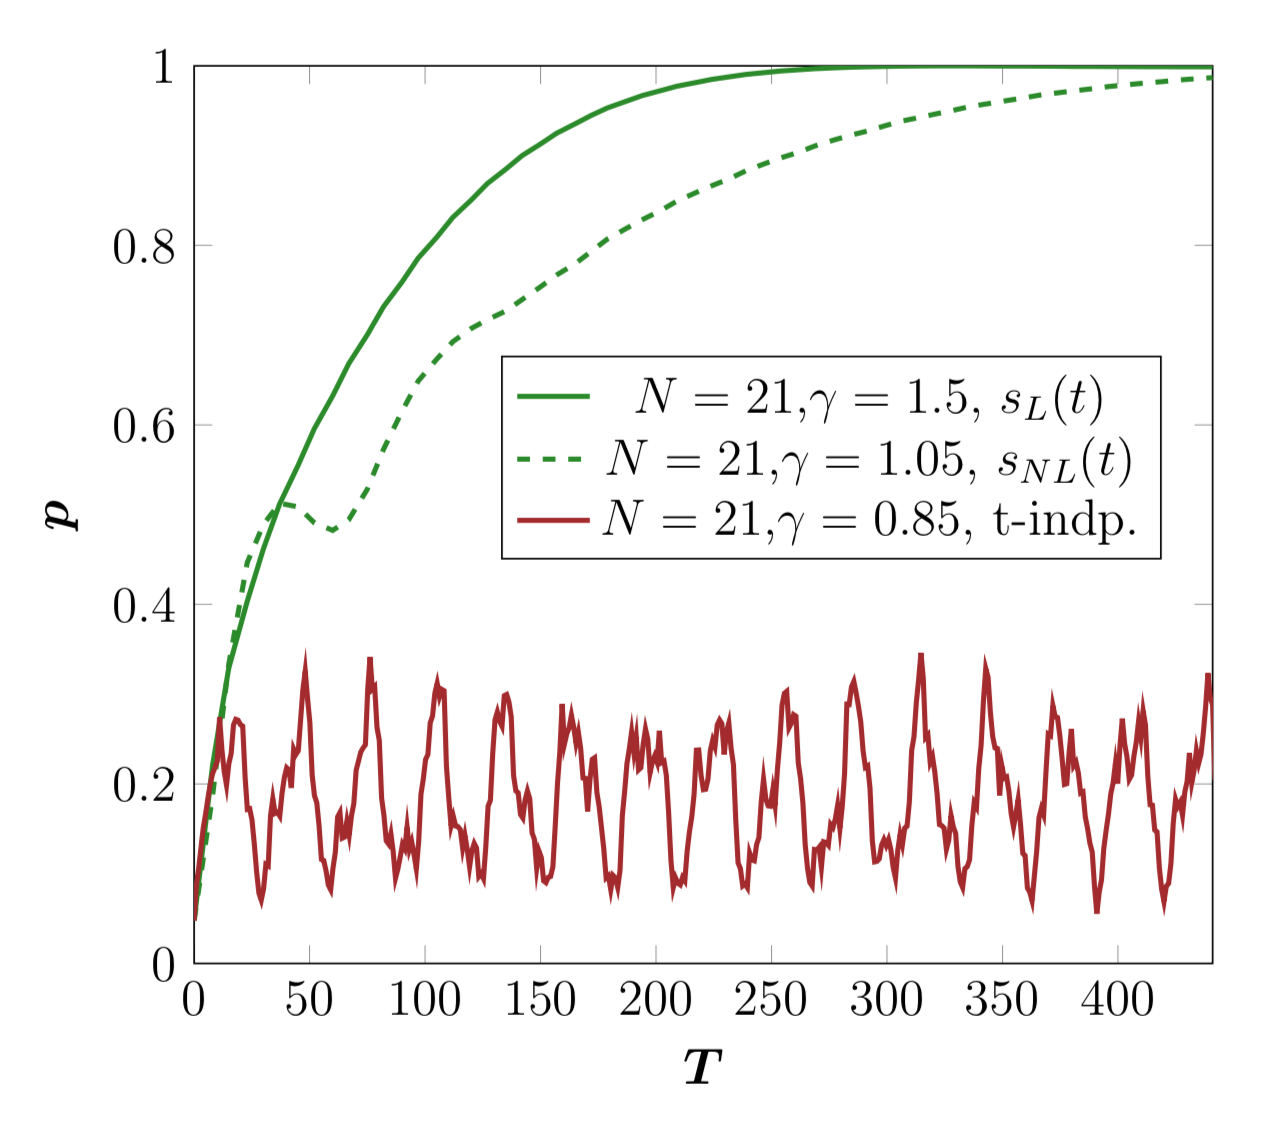
\includegraphics[width=\textwidth]{localization.png}
	\end{column}
\end{columns}

\begin{itemize}
	\item Time-dependent approach produces high probability ($p<1$) in much less time than for $p=1$ \\(e.g. for $s_L(t)$ $p=1$ at $T=300$, $p=0.9$ at $T=150$)
\end{itemize}



\end{frame}

%------------------------------------------------

\begin{frame}
\frametitle{Cycle graph: search \\ \normalsize $\blacksquare$ Multiple runs search with constraint on $T$}

\begin{itemize}
	\item We consider the multiple runs for one search approach\\(*) Time-dependent is not optimized on $T$ \\(*) Time-independent is an imperfect search
	\item We introduce a \bb{new quantity} $\tau$ in order to compare the two approaches
\end{itemize}
\vspace{0.3cm}

\centering
\begin{tcolorbox}[width=4.0cm, colframe=darkblue, colback=white, halign=center, left=1pt, right=1pt, top=-11pt, bottom=1pt]
	\begin{equation*}
		\tau = \min \Big(\frac{T}{p}\Big)_{T>T_{\min}, \gamma}
	\end{equation*}
\end{tcolorbox}


\vspace{0.3cm}
\begin{itemize}
	\item $T_{\min}$ is a constraint on the minimum time
	\item $T_{\min} = \frac{\pi}{2}\sqrt{N}$
\end{itemize}
\end{frame}

%------------------------------------------------

\begin{frame}
\frametitle{Cycle graph: search (2) \\ \normalsize $\blacksquare$ Time-dependent performs better than time-independent}

\begin{columns}
	\begin{column}[T]{0.5\textwidth}
		\begin{itemize}
			\item Similar performance for small $N$ ($<35$)
			\item Time-dependent approach wins for large $N$
			\item Non-linear $s(t)$ performs slightly better than the linear one
		\end{itemize}
		\vspace{-0.3cm}
		
	\end{column}

	\begin{column}[T]{0.5\textwidth}
		\vspace{-0.5cm}
		\begin{figure}
			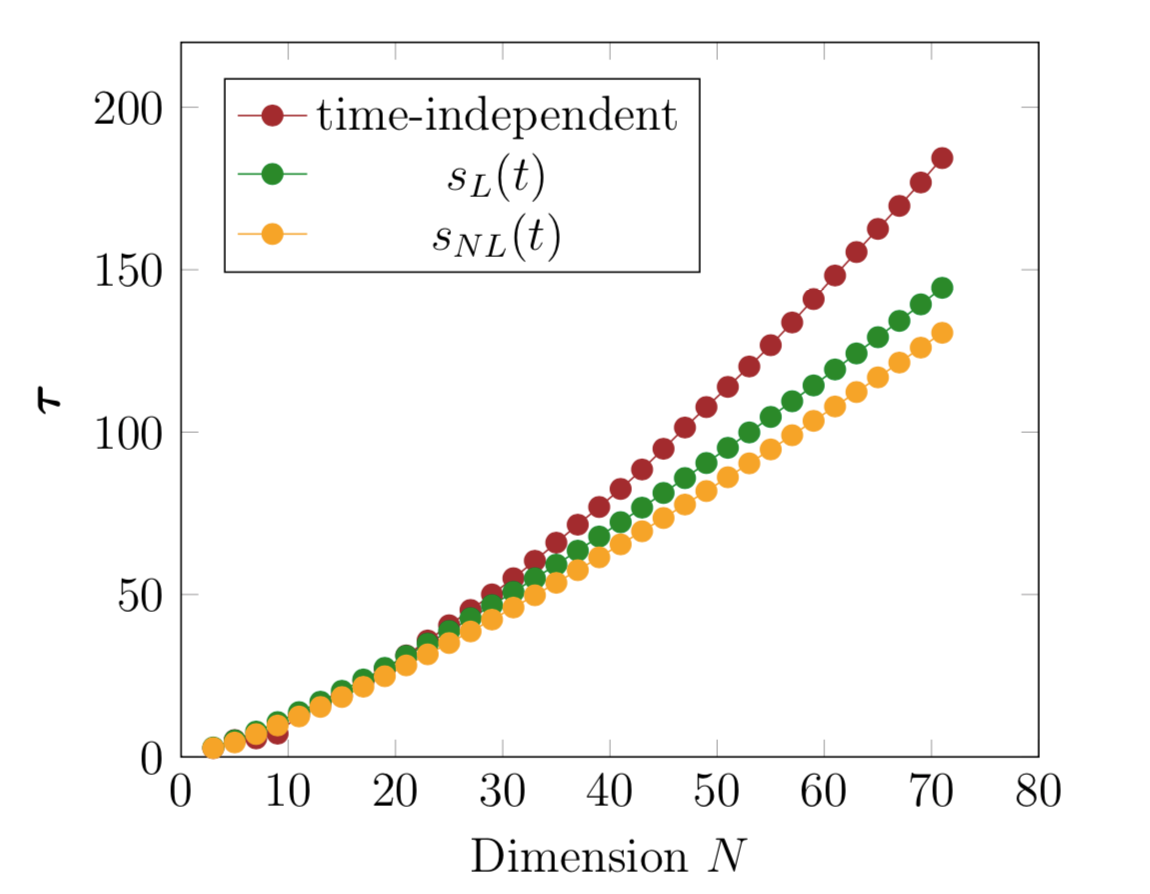
\includegraphics[width=\textwidth]{tau.png}
		\end{figure}
	\end{column}

\end{columns}
\end{frame}

%------------------------------------------------

\begin{frame}
\frametitle{Cycle graph: robustness \\ \normalsize $\blacksquare$ Time-dependent approach with linear $s(t)$ is the most robust}

\begin{itemize}
	\item Robustness is evaluated for a $T$, $\gamma$ variation of $2$ \bb{grid blocks}
	\item \bb{$\gamma$-Robustness}: time-dependent is best, with linear $s(t)$ the most robust
	\item \bb{$T$-Robustness}: surprisingly the time-independent is more robust for large $N$, although the values are very similar
\end{itemize}

\begin{columns}
	\begin{column}[T]{0.4\textwidth}
		\begin{figure}
		\centering
			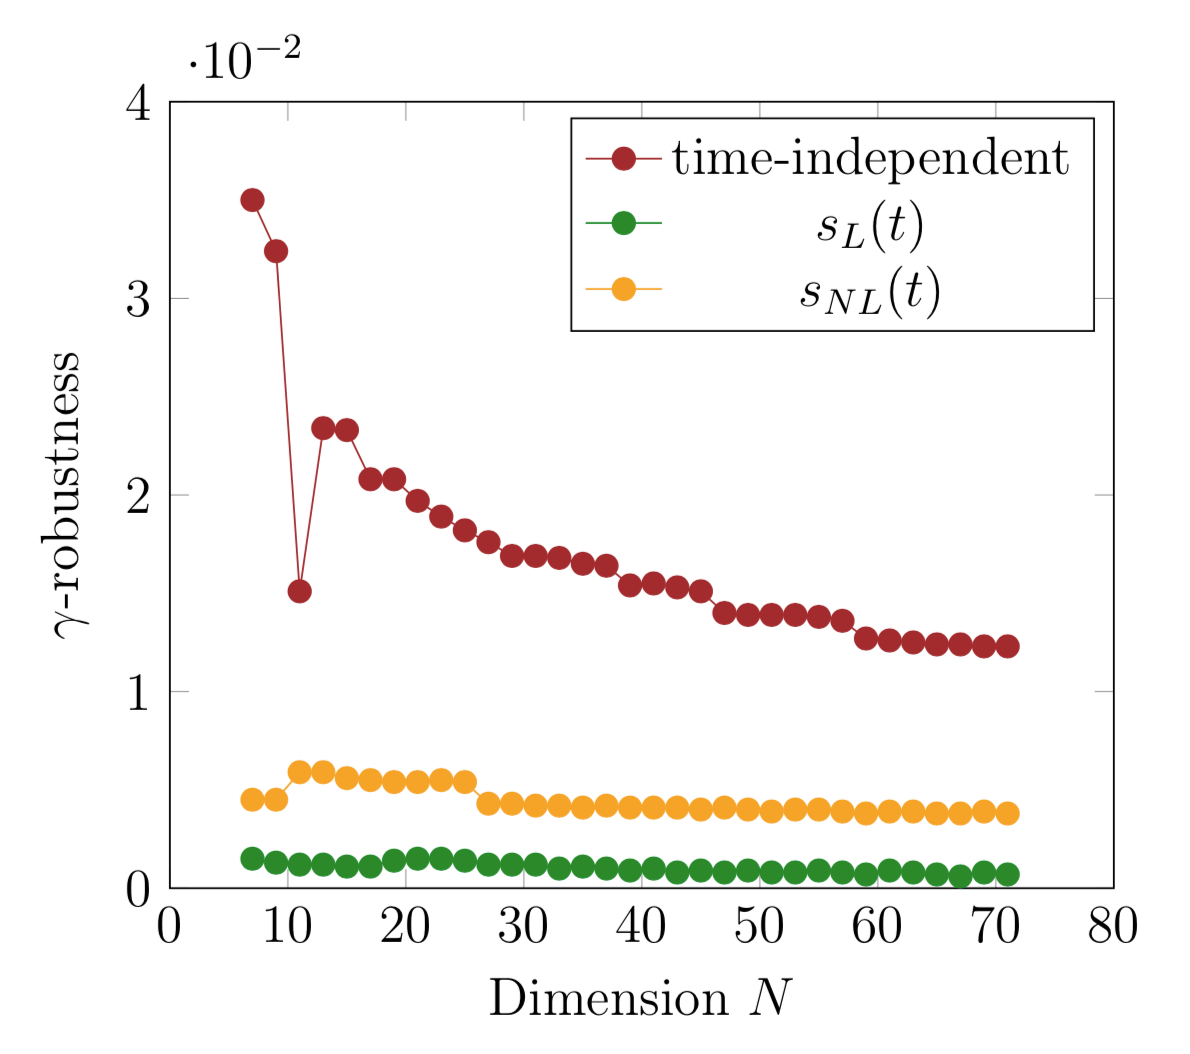
\includegraphics[width=\textwidth]{gamma_robustness.png}
		\end{figure}
	\end{column}

	\begin{column}[T]{0.4\textwidth}
		\begin{figure}
		\centering
			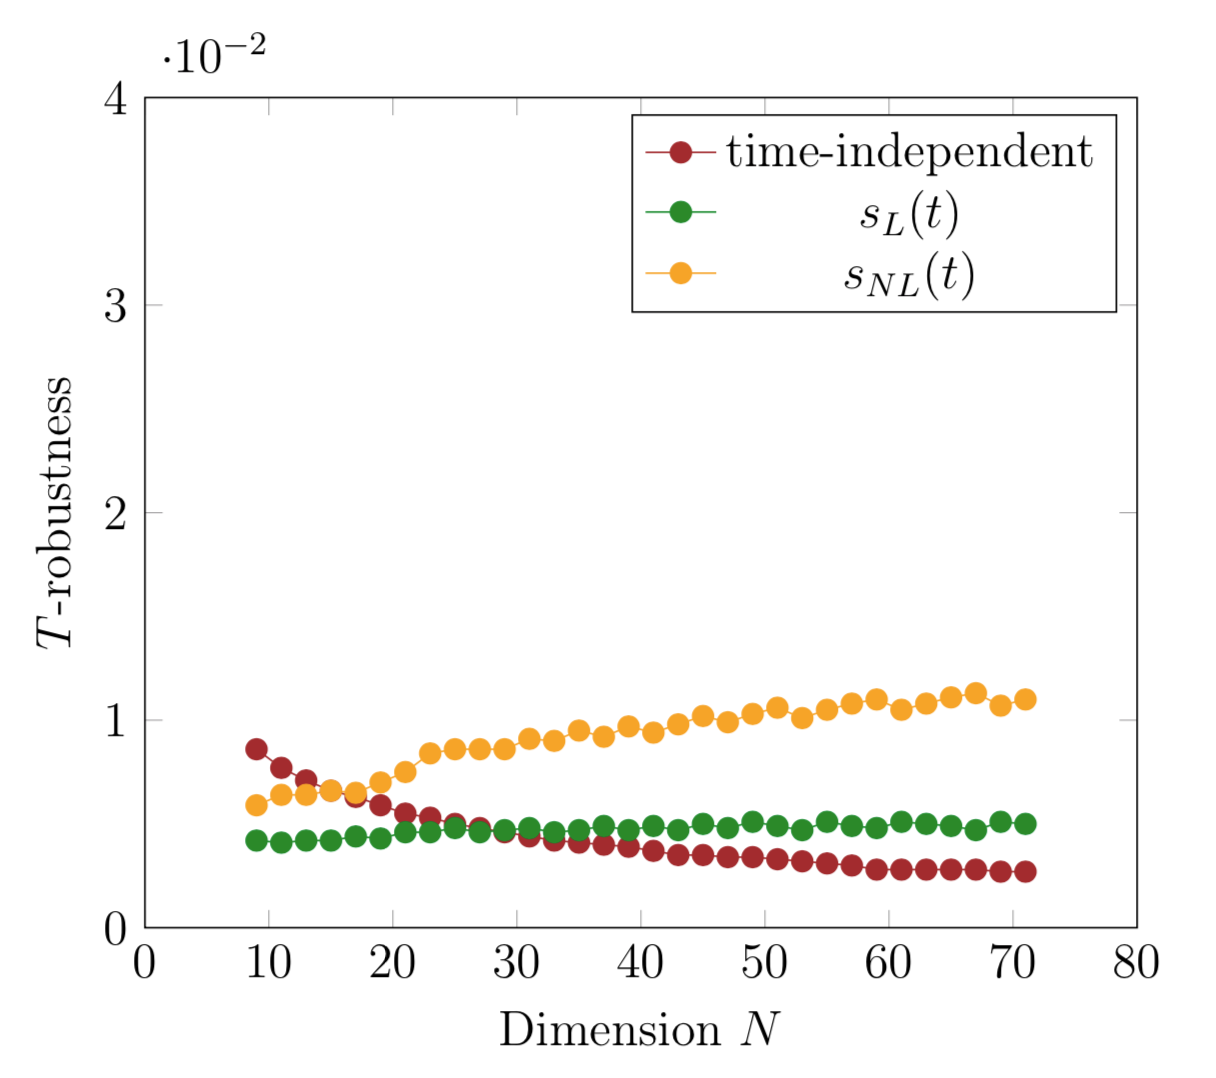
\includegraphics[width=\textwidth]{time_robustness.png}
		\end{figure}
	\end{column}

\end{columns}
\end{frame}

%------------------------------------------------

\begin{frame}
\frametitle{Complete graph: probability and qualitative robustness \\ \normalsize $\blacksquare$ Time-dependent is more robust but with much worse time scaling}

\begin{itemize}
	\item For completeness we study the complete graph
	\item We do not expect to be able to improve an already optimal approach
	\item We might get some insights on the performance of our algoritihm 
	\item We study the \bb{qualitative robustness} (in figure $N=51$)
\end{itemize}

\begin{figure}
	\centering
	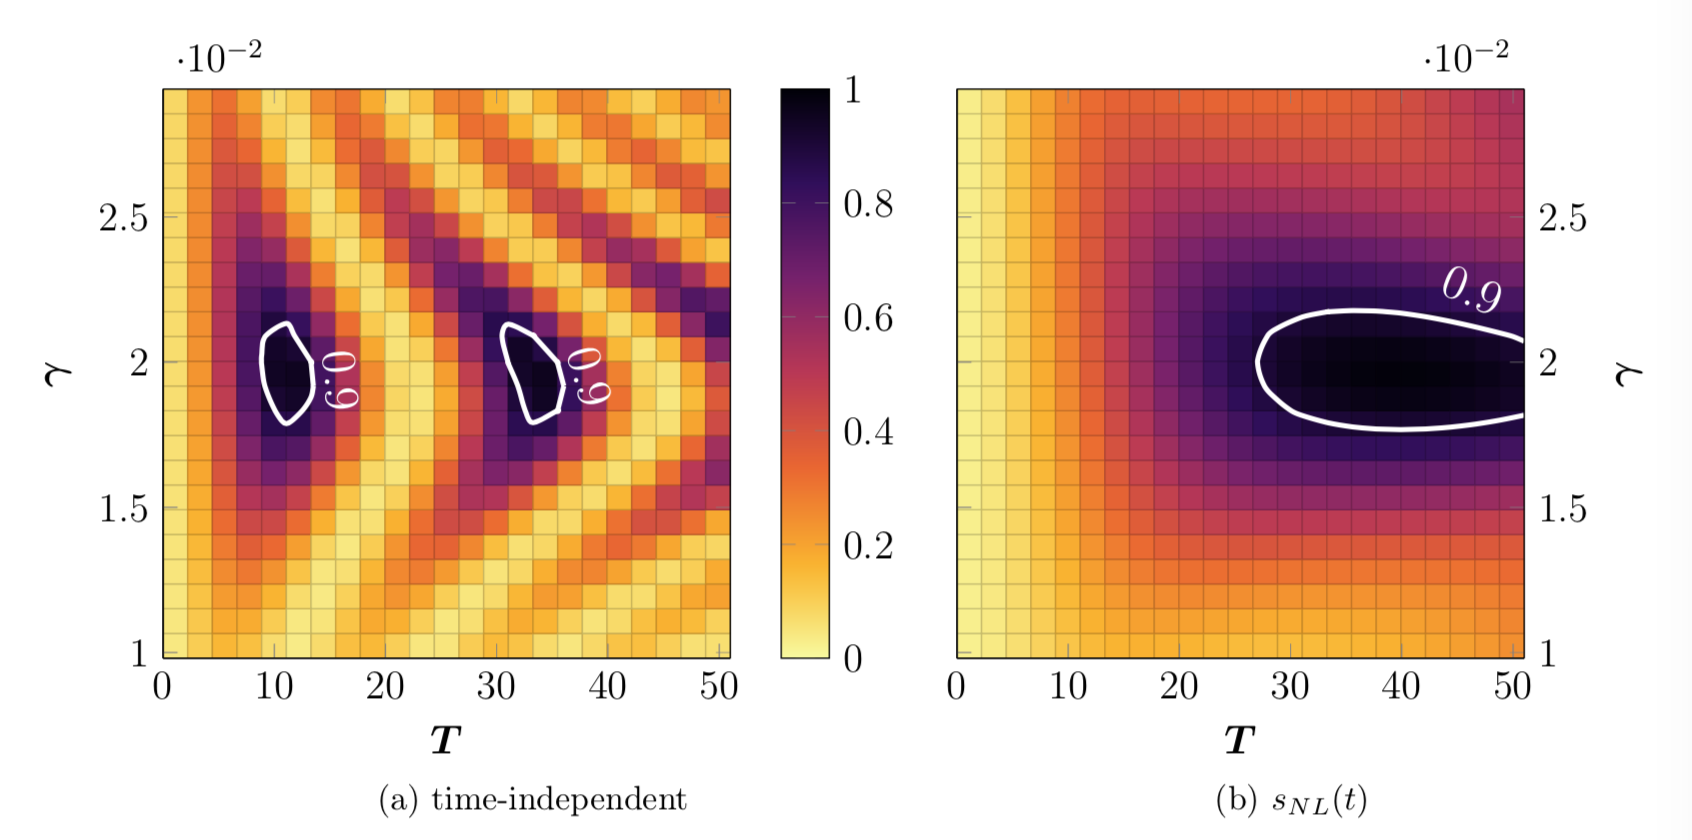
\includegraphics[width=0.8\textwidth]{complete_heatmap.png}	
\end{figure}

\end{frame}

%------------------------------------------------

\begin{frame}
\frametitle{The choice of $s(t)$ is crucial}

\begin{itemize}
	\item As already mentioned the choice of $s(t)$ is crucial
	\item Improvements on the performance come from the choice of the optimal $s(t)$ 
	\item Linear $s(t)$ performs \bb{worse} than \bb{classical} algorithms (in figure $N=51$)
\end{itemize}

\begin{figure}
	\centering
	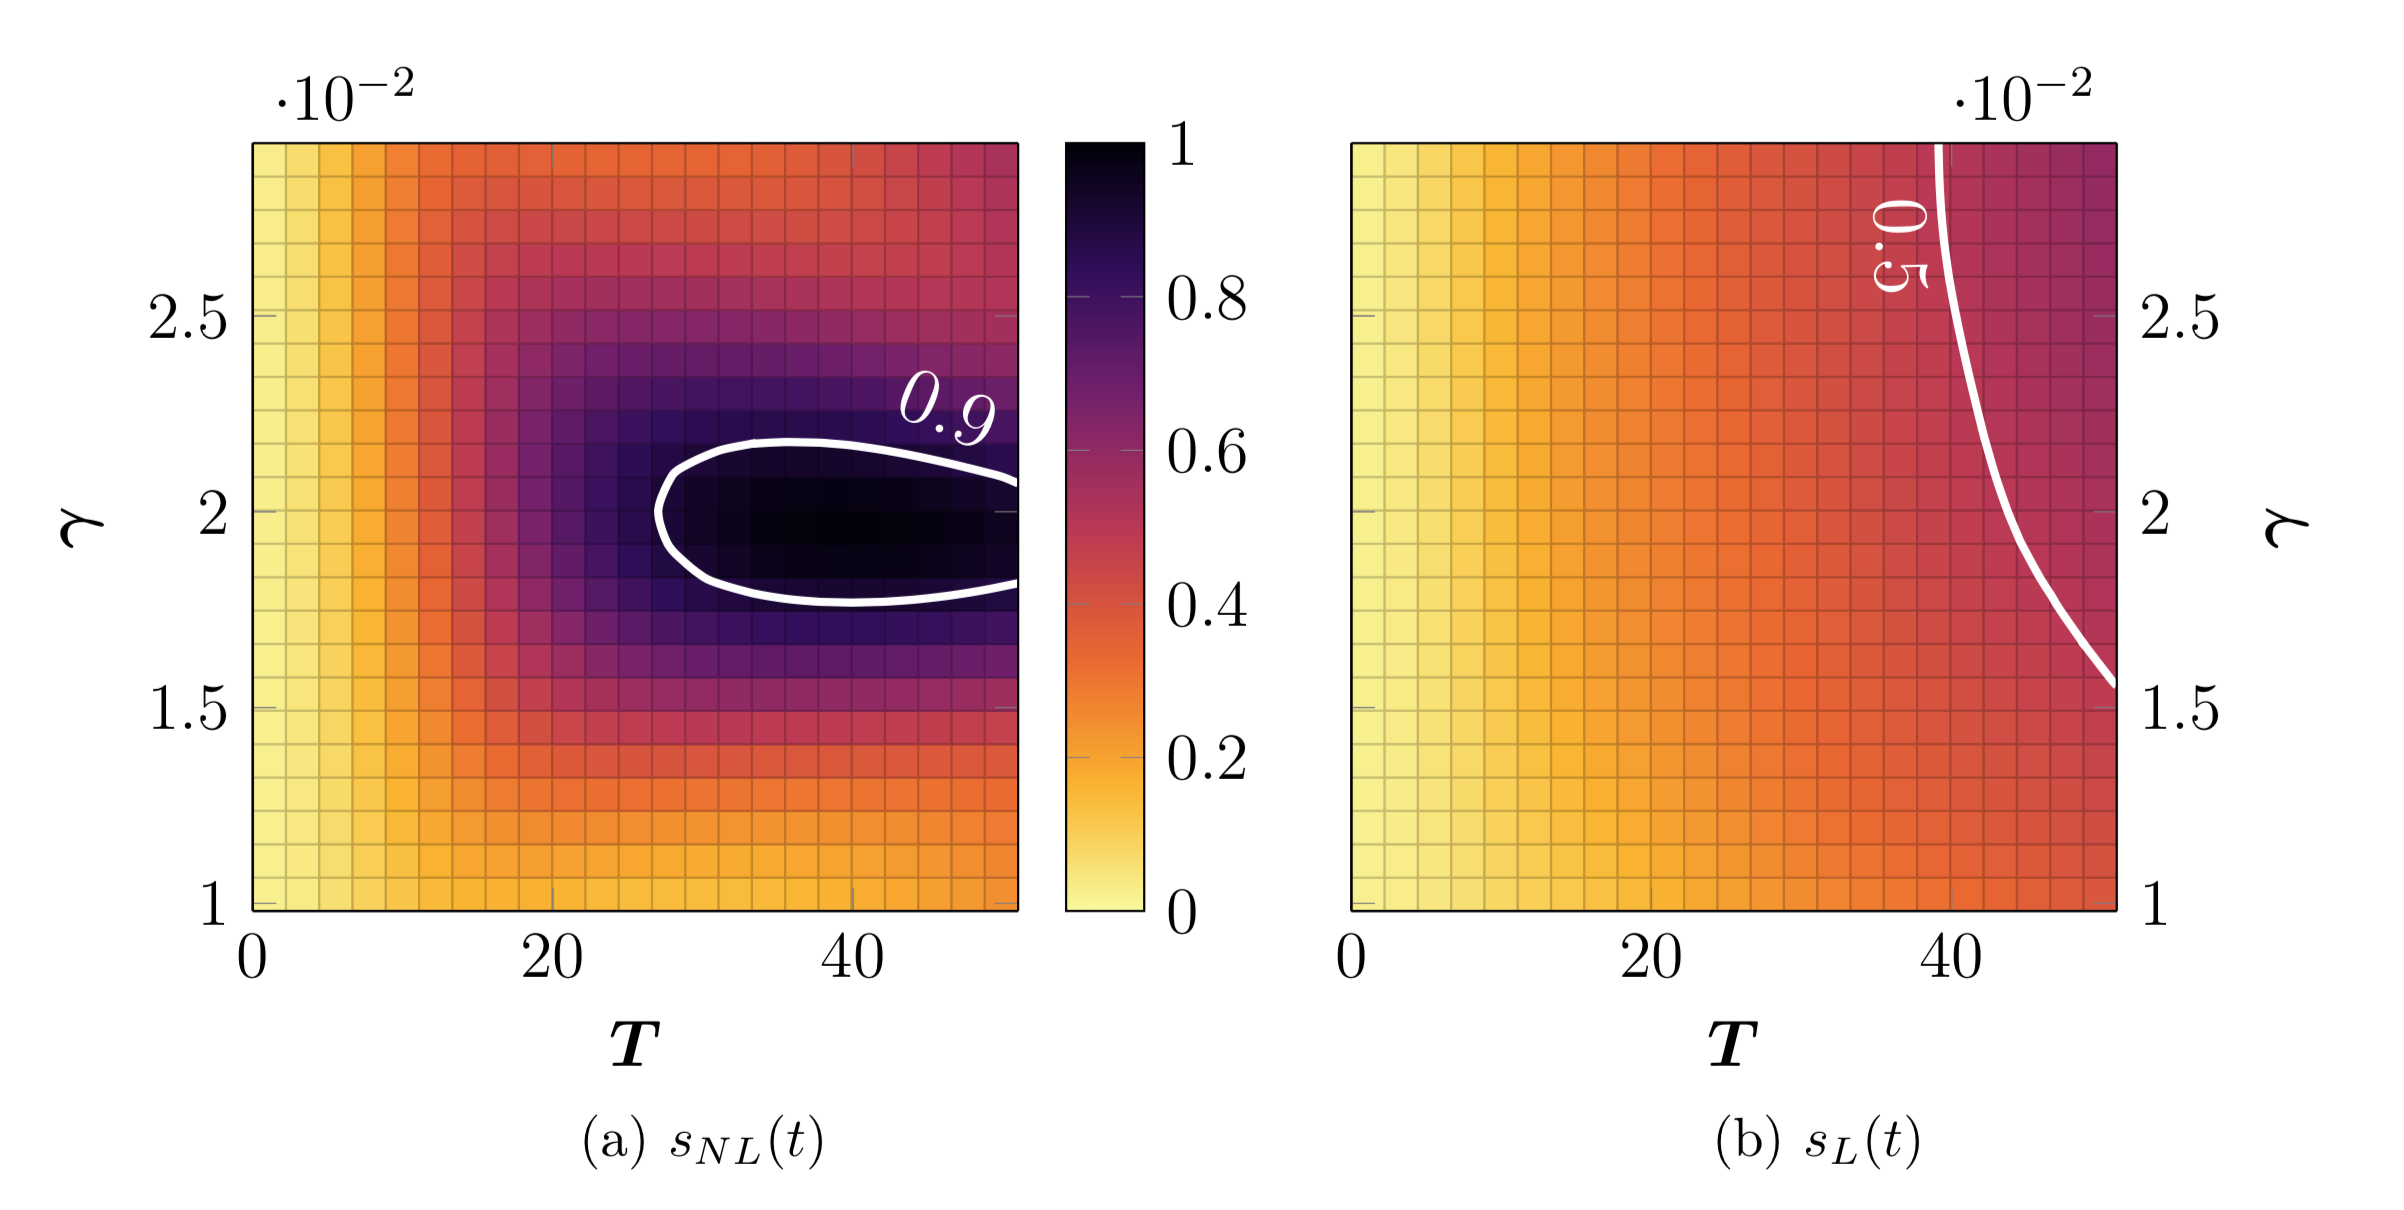
\includegraphics[width=0.8\textwidth]{complete_heatmap_time_dependent.png}
\end{figure}
\end{frame}

%------------------------------------------------

\begin{frame}
\frametitle{What have we learned?}

\centering 
Results from applying the time-dependent Hamiltonian algorithm
\vspace{0.2cm} 
\begin{columns}

	\begin{column}[T]{0.4\textwidth}
	{
	\centering
	\begin{tcolorbox}[width=2.5cm, colframe=darkblue, colback=white, halign=center, left=0pt, right=0pt, top=2pt, bottom=2pt]
	\bb{Cycle graph\\} 
	\end{tcolorbox}
	}
	\begin{itemize}
		\item Shows localization properties
		\item Is more robust
		\item Better search performance overall
		\item Non-linear $s(t)$ performs better but is less robust
	\end{itemize}

	\end{column}

	\begin{column}[T]{0.4\textwidth}
	{
	\centering
	\begin{tcolorbox}[width=3.5cm, colframe=darkblue, colback=white, halign=center, left=0pt, right=0pt, top=2pt, bottom=2pt]
	\bb{Complete graph} 
	\end{tcolorbox}
	}
	\begin{itemize}
		\item Is (qualitatively) more robust
		\item Performs much worse than Grover
		\item Performs better than classical
		\item Shows that $s(t)$ has great impact on the performance
	\end{itemize}

	\end{column}

\end{columns}

\end{frame}

%------------------------------------------------

\begin{frame}
\frametitle{What is next?}

\begin{itemize}
	\item The application of the algorithm to the complete graph \\suggests that \bb{improvements} on the performance come\\ from the choice of the \bb{optimal $s(t)$}
\end{itemize}
\vspace{0.3cm}
\begin{itemize}
	\item Application to \bb{different graph topologies}
\end{itemize}
\end{frame}

%------------------------------------------------

\begin{frame}
\centering
\vspace{0.5cm}
\bb{Thanks for your attention}
\end{frame}

%----------------------------------------------------------------------------------------

\end{document} 